\begin{blocksection}
\question Draw the environment diagram that results from running the following code.
\begin{lstlisting}
ghost = [1, 0,[3], 1]
def boo(spooky):
  ghost.append(spooky.append(ghost))
  spooky = spooky[ghost[2][1][1]]
  ghost[:].extend([spooky])
  spooky = [spooky] + [ghost[spooky - 1].pop()] 
  ghost.remove(ghost.remove(1))
  spooky += ["Happy Halloween!"]
  return spooky
pumpkin = boo(ghost[2])
\end{lstlisting}

\begin{solution}[1in]
  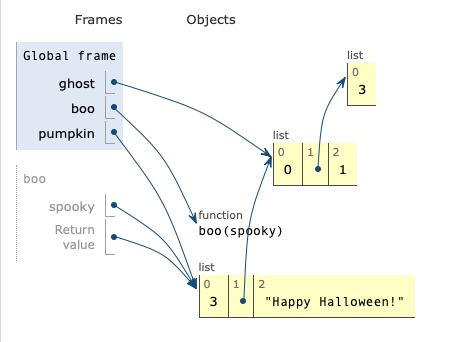
\includegraphics[width=.5\textwidth]{spooky-list_sol.png}
  \newline
  \href{https://tinyurl.com/2zxktfjb}{PythonTutor Link: https://tinyurl.com/2zxktfjb} 
\end{solution}
\begin{guide}
\textbf{Teaching Tips}
\newline
  Explanations for some tricky steps:
  \begin{itemize}
    \item Line 3: \lstinline{append} returns \lstinline{None}, so \lstinline{ghost} is appended to \lstinline{spooky} by inserting a new pointer to the list bound to \lstinline{ghost} at fourth index of \lstinline{spooky} and then \lstinline{None} is appended to \lstinline{ghost}
    \item Line 5: This does nothing because the value of this expression is never assigned to a variable. List slicing creates a copy of a list that is immediately deleted
    \item Line 6: Pop returns the last element of the original value of spooky. Since we use \lstinline{=} and then \lstinline{+} instead of \lstinline{+=}, a new list is created
    \item Line 7: \lstinline{remove} deletes the first element with a given value, so the first instance of 1 is deleted. \lstinline{remove} returns \lstinline{None}, so the outer call to \lstinline{remove} gets rid of the \lstinline{None} element of \lstinline{ghost}
    \item Line 8: \lstinline{+=} mutates \lstinline{spooky} instead of creating a new list 
    \item Go over the difference between shallow and deep copying.
    \begin{itemize}
			\item Shallow copying is when you copy each element as is; i.e. elements which were pointers to a list still point to the same list in the copy.
			\item Deep copying is when you copy each element within each sublist; i.e. the new elements which are pointers point to brand-new created lists.
			\item In general, most operators involving Python lists perform shallow copying: i.e. slicing, list(...), etc. 
    \end{itemize}
    \item Use box and pointer diagrams in your environment diagram for lists.
  \end{itemize}
\end{guide}
\end{blocksection}